\documentclass[,jou, a4paper,floatsintext]{apa6}
\usepackage{lmodern}
\usepackage{amssymb,amsmath}
\usepackage{ifxetex,ifluatex}
\usepackage{fixltx2e} % provides \textsubscript
\ifnum 0\ifxetex 1\fi\ifluatex 1\fi=0 % if pdftex
  \usepackage[T1]{fontenc}
  \usepackage[utf8]{inputenc}
\else % if luatex or xelatex
  \ifxetex
    \usepackage{mathspec}
  \else
    \usepackage{fontspec}
  \fi
  \defaultfontfeatures{Ligatures=TeX,Scale=MatchLowercase}
\fi
% use upquote if available, for straight quotes in verbatim environments
\IfFileExists{upquote.sty}{\usepackage{upquote}}{}
% use microtype if available
\IfFileExists{microtype.sty}{%
\usepackage{microtype}
\UseMicrotypeSet[protrusion]{basicmath} % disable protrusion for tt fonts
}{}
\usepackage{hyperref}
\hypersetup{unicode=true,
            pdftitle={Analysis of Open Data and Computational Reproducibility in Registered Reports in Psychology},
            pdfauthor={Pepijn Obels, Daniel Lakens, Nicholas A. Coles, Jaroslav Gottfried, \& Seth Ariel Green},
            pdfkeywords={reproducibility, Registered Reports, data sharing, open science},
            pdfborder={0 0 0},
            breaklinks=true}
\urlstyle{same}  % don't use monospace font for urls
\usepackage{graphicx,grffile}
\makeatletter
\def\maxwidth{\ifdim\Gin@nat@width>\linewidth\linewidth\else\Gin@nat@width\fi}
\def\maxheight{\ifdim\Gin@nat@height>\textheight\textheight\else\Gin@nat@height\fi}
\makeatother
% Scale images if necessary, so that they will not overflow the page
% margins by default, and it is still possible to overwrite the defaults
% using explicit options in \includegraphics[width, height, ...]{}
\setkeys{Gin}{width=\maxwidth,height=\maxheight,keepaspectratio}
\IfFileExists{parskip.sty}{%
\usepackage{parskip}
}{% else
\setlength{\parindent}{0pt}
\setlength{\parskip}{6pt plus 2pt minus 1pt}
}
\setlength{\emergencystretch}{3em}  % prevent overfull lines
\providecommand{\tightlist}{%
  \setlength{\itemsep}{0pt}\setlength{\parskip}{0pt}}
\setcounter{secnumdepth}{0}
% Redefines (sub)paragraphs to behave more like sections
\ifx\paragraph\undefined\else
\let\oldparagraph\paragraph
\renewcommand{\paragraph}[1]{\oldparagraph{#1}\mbox{}}
\fi
\ifx\subparagraph\undefined\else
\let\oldsubparagraph\subparagraph
\renewcommand{\subparagraph}[1]{\oldsubparagraph{#1}\mbox{}}
\fi

%%% Use protect on footnotes to avoid problems with footnotes in titles
\let\rmarkdownfootnote\footnote%
\def\footnote{\protect\rmarkdownfootnote}


  \title{Analysis of Open Data and Computational Reproducibility in Registered Reports in Psychology}
    \author{Pepijn Obels\textsuperscript{1}, Daniel Lakens\textsuperscript{1}, Nicholas A. Coles\textsuperscript{2}, Jaroslav Gottfried\textsuperscript{3}, \& Seth Ariel Green\textsuperscript{Code Ocean}}
    \date{}
  
\shorttitle{Reproducing Registered Reports}
\affiliation{
\vspace{0.5cm}
\textsuperscript{1} Eindhoven University of Technology, The Netherlands\\\textsuperscript{2} University of Tennessee, Knoxville, USA\\\textsuperscript{3} Masaryk University, Brno, Czech Republic}
\keywords{reproducibility, Registered Reports, data sharing, open science\newline\indent Word count: 4926}
\usepackage{csquotes}
\usepackage{upgreek}
\captionsetup{font=singlespacing,justification=justified}

\usepackage{longtable}
\usepackage{lscape}
\usepackage{multirow}
\usepackage{tabularx}
\usepackage[flushleft]{threeparttable}
\usepackage{threeparttablex}

\newenvironment{lltable}{\begin{landscape}\begin{center}\begin{ThreePartTable}}{\end{ThreePartTable}\end{center}\end{landscape}}

\makeatletter
\newcommand\LastLTentrywidth{1em}
\newlength\longtablewidth
\setlength{\longtablewidth}{1in}
\newcommand{\getlongtablewidth}{\begingroup \ifcsname LT@\roman{LT@tables}\endcsname \global\longtablewidth=0pt \renewcommand{\LT@entry}[2]{\global\advance\longtablewidth by ##2\relax\gdef\LastLTentrywidth{##2}}\@nameuse{LT@\roman{LT@tables}} \fi \endgroup}

\authornote{This work was supported by the Netherlands Organization for Scientific Research (NWO) VIDI grant 452-17-013. All code used to create this manuscript is provided in an OSF repository at \url{https://osf.io/suqz3/}.

Correspondence concerning this article should be addressed to Daniel Lakens, ATLAS 9.402, 5600 MB, Eindhoven, The Netherlands. E-mail: \href{mailto:D.Lakens@tue.nl}{\nolinkurl{D.Lakens@tue.nl}}}

\abstract{
Ongoing technological developments have made it easier than ever before for scientists to share their data, materials, and analysis code. Sharing data and analysis code makes it easier for other researchers to re-use or check published research. These benefits will only emerge if researchers can reproduce the analysis reported in published articles, and if data is annotated well enough so that it is clear what all variables mean. Because most researchers have not been trained in computational reproducibility, it is important to evaluate current practices to identify practices that can be improved. We examined data and code sharing, as well as computational reproducibility of the main results, without contacting the original authors, for Registered Reports published in the in psychological literature between 2014 and 2018. Of the 62 articles that met our inclusion criteria, data was available for 40 articles, and analysis scripts for 37 articles. For the 35 articles that shared both data and code and performed analyses in SPSS, R, Python, MATLAB, or JASP, we could run the scripts for 31 articles, and reproduce the main results for 20 articles. Although the articles that shared both data and code (35 out of 62, or 56\%) and articles that could be computationally reproduced (20 out of 35, or 57\%) was relatively high compared to other studies, there is clear room for improvement. We provide practical recommendations based on our observations, and link to examples of good research practices in the papers we reproduced.


}

\begin{document}
\maketitle

Researchers are currently exploring ways to make science more open and transparent. Among novel developments such as pre-registration, pre-prints, and open peer review, an increasing number of journals, funders, and researchers are beginning to expect that data, materials, and analysis code will be shared by default with scientific publications (e.g., (Morey et al., 2016). Sharing data and analysis code with scientific publications allows others to more easily reproduce, check, and build on existing work. This requires the development of new skills and best practices, since most scientists have not received training in how to make their work reproducible. It is important to evaluate how data and code are currently being shared, and how easy it is to reproduce analyses reported in the published literature, to learn what can be improved. With this goal in mind, we computationally reproduced the main results of Registered Reports published in the psychological literature.

It is desirable that research is reproducible. Data availability has the potential to make science more efficient by facilitating the re-use of data. The availability of analysis code makes it possible for peers to check and correct published findings. According to Kitzes, Turek, and Deniz (2017), computational reproducibility means that ''a second investigator (including the original researcher in the future) can recreate the final reported results of the project, including key quantitative findings, tables, and figures, given only a set of files and written instructions.'' For scientific research to be computationally reproducible, the data and code needs to be shared.

However, the availability of data and code in itself is not enough. Articles need to link to these materials so that readers know where to find them. Preferably, the data should be available in a format that can be read by open source software. Variables must be described and labeled (e.g., in a codebook), and code should be annotated. Finally, the results reported in the scientific manuscript should be reproducible, which means the data and code can be used to compute the results that are reported in the published article.

Recently, scholars have started to empirically examine the extent to which data is shared with published articles, and, if so, whether it was possible to reproduce the data analysis reported in the published article. Hardwicke et al. (2018) examined the reproducibility of 35 articles published in the journal \emph{Cognition}. Eleven articles could be reproduced without assistance from the original authors, and 13 articles contained at least one outcome that could not be reproduced even with author assistance. The authors estimated that it took between 2-25 hours to reproduce the reported results per article, but they did not record the exact time. Stockemer, Koehler, and Lentz (2018) analyzed reproducibility in all articles published in 2015 in three political science journals. They emailed authors for the code and data, and found that for 71 articles for which they received code and data, one could not be reproduced due to a lack of a software license, and 16 articles could not be reproduced with access to the required software. For the remaining articles, 32 could be exactly reproduced, 19 could be reproduced with slight differences, and 3 articles yielded significantly different results. Stodden, Seiler, and Ma (2018) analyzed data availability in the journal \emph{Science} in 2011-2012 and found that 26 of 204 (or 13\%) of articles provided information to retrieve data and/or code without contacting the authors. For all datasets they acquired after e-mailing authors for data and code, 26\% was estimated to be computationally reproducible. These studies reveal that there is clear room for improvement in how reproducible published articles are.

We set out to examine the data availability and reproducibility in Registered Reports published in psychological science. Our main interest was to examine the computational reproducibility of the main analyses reported in published articles, without contacting the original authors. One of the main benefits of sharing data and code with an article (compared to making these files available upon request) is that results can be reproduced, and data reused even if the original author can no longer be reached.

Registered Reports are a novel development in psychology. Before data collection commences, the introduction and methods are peer-reviewed, after which authors can receive an \enquote{in-principle acceptance}. This means the article will be published as long as the authors follow their preregistered data collection and analysis plan (Chambers, Feredoes, Muthukumaraswamy, \& Etchells, 2014; Nosek \& Lakens, 2014). The population of Registered Reports in psychology is still relatively small (91 Registered Reports had been published as of February 22, 2018), which makes it possible to examine it in full.

The novelty of Registered Reports may attract early adopters who are also exploring other novel developments aimed at improving research practices in psychology, such as data and code sharing. We hypothesized that researchers who publish Registered Reports would also be likely to share data and code in public repositories, and to embrace computational reproducibility. In line with our hypothesis, 43 out of 62 articles in our final dataset shared at least some of the data and code (69.40\%). In comparison, after the journal \emph{Cognition} introduced a mandatory data sharing policy, 136 out of 174 articles (78.2\%) had a data availability statement, 85 of 174 articles (49\%) had reusable data, and only 18 out of 174 articles (10.3\%) provided the analysis code (Hardwicke et al., 2018). To evaluate the reproducibility of findings published in Registered Reports, we examined if data could be located, were available at the indicated location, could be opened in open-source or accessible software, were documented well enough to be understandable, and could be used to reproduce the main analyses reported in the published manuscript.

\hypertarget{the-current-research}{%
\subsubsection{The Current Research}\label{the-current-research}}

Our main objective was to examine how reusable data and code underlying Registered Reports are, based purely on the information provided in the published literature. We examined how many authors voluntarily shared data and code, and the extent to which we could reproduce reported analyses without contacting the original authors. While reproducing the results reported in Registered Reports, we kept track of factors that facilitated reproducibility or that made reproducing the result more difficult. We report these qualitative findings with an aim to highlight how current practices can be improved.

\hypertarget{method}{%
\subsubsection{Method}\label{method}}

To find Registered Reports published in psychology we drew from a database of registered reports maintained by the Center for Open Science.\footnote{\url{https://www.zotero.org/groups/479248/osf/items/collectionKey/KEJP68G9}} At the start of this project (06-05-2018) this database consisted of 118 published Registered Reports. Eighty-one articles in this database were published in the psychological literature. We limited our analysis to studies performed by single groups, since such articles are most representative of the researchers currently work, and excluded 7 large scale collaborations where dedicated team members were responsible for making the analysis reproducible, such as Registered Replication Reports (Hagger et al., 2016) and Many Labs projects (Klein et al., 2014, 2018). Upon further inspection of the 72 papers left in the dataset, it turned out that 10 were not formally Registered Reports. This left 62 studies in our sample. When evaluating whether we could reproduce the original results, we limited ourselves to statistical software packages that we had experience with (R, SPSS, Python, MATLAB, and JASP) and excluded studies that required expertise in software packages we are not trained in (e.g., dedicated EEG software), which led to the exclusion of 1 additional study.

\hypertarget{results}{%
\subsubsection{Results}\label{results}}

We set out to reproduce the 62 papers that met our inclusion criteria. For each article we coded whether the data and code were (a) linked, (b) available, (c) not software-specific, (d) understandable, and (e) reproducible. These five categories were inspired by FAIR data principles (Wilkinson et al., 2016) that address the findability, accessibility, interoperability, and reusability of data and code, but we did not explicitly code whether papers adhered to the exact definitions of the four FAIR principles. Our main aim was to examine the reproducibility of results, while adhering to FAIR criteria requires meeting more stringent requirements, for example concerning the presence of metadata (which is missing for practically all datasets). We considered data and code to be linked when the manuscript included a unique link to the data and scripts. Ideally, such a link consists of a stable digital object identifier (DOI). A hyperlink to a website that contains the data and script also suffices, although normal hyperlinks are known to break over time (Gertler \& Bullock, 2017).

Of the 62 papers, 45 linked to data and/or code that were part of the article. Linking to data or code does not mean the data is actually available, and not linking to data in an article does not mean data is unavailable. For one article the link no longer worked (highlighting the need to use a stable DOI when linking to data). For three articles the link still worked, but there was no data at the linked destination. For three articles where there was no link to the data in the article, we were nevertheless able to find data on the Open Science Framework when searching for the title of the paper. For one paper the data was linked but not available, as the data was embargoed until a future date. Altogether, some data or code was available for 43 out of 62 papers. For 37 articles the available code contained the statistical analyses, and for 40 all the required data files were available to reproduce the reported results (for 35 articles both data and code were available.

We also coded the extent to which data and code was specific to software that was not freely available. When open source software is used, the analyses can be reproduced by anyone with a computer and internet, regardless of whether they have bought the same software package. When proprietary software is used, results might still be reproducible by anyone, but it could require more effort to do so. For example, SPSS produces proprietary .sav and .sps files. However, .sav files can be opened in R, and .sps files can be opened by a text editor and the code can be rewritten, as long the code is annotated well enough to be recoded into R. Note that we had access to SPSS and therefore reproduced the analyses using the original .sps scripts where available. The data files of one article where an EEG study was reported consisted of .eeg, .vhdr, and vmrk files required dedicated EEG software and could not be reproduced (we could also not find the analysis code for this article).

\begin{figure*}
\begin{center}
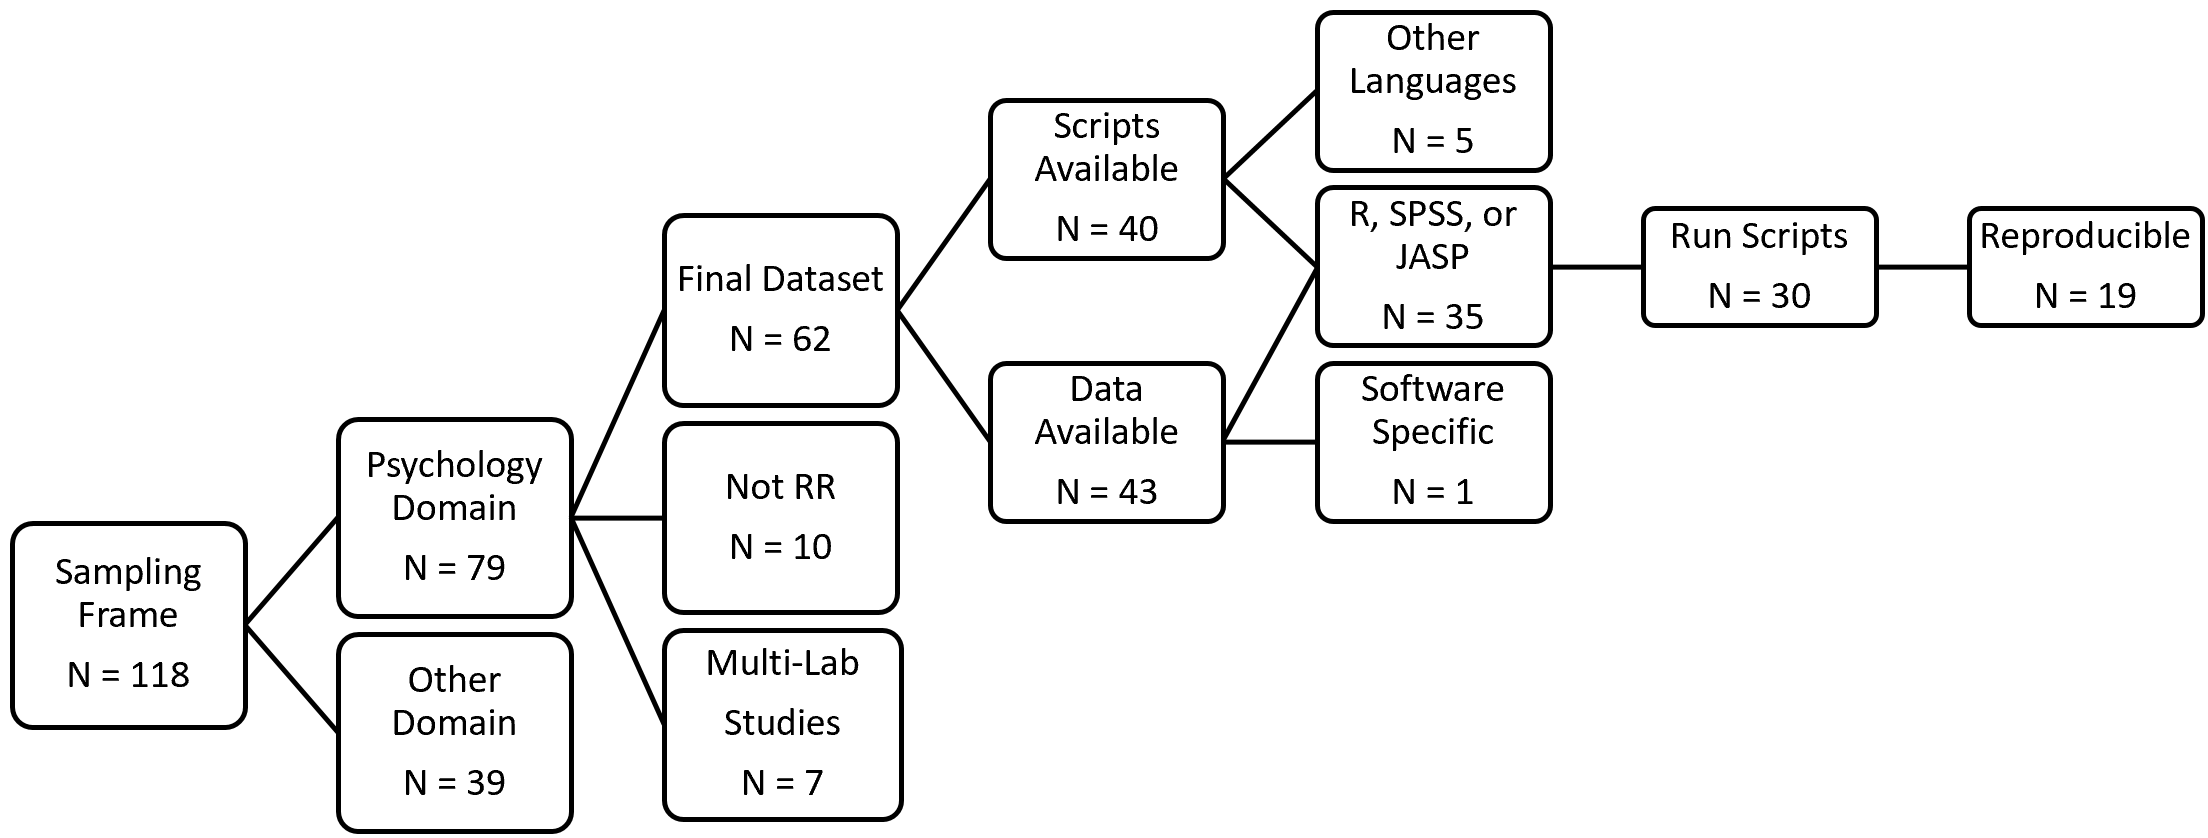
\includegraphics[width=\textwidth]{fig1.png}

\caption{Of all articles in the Registered Report database 79 were psychology related, and 62 were registered reports not part of a multi-lab Registered Replication Report. Of these 62 papers, 45 linked to the data or code. After searching the OSF, data or code was available for 43 studies, of which 39 articles used SPSS, R, Matlab, Python, or JASP. Of the 62 papers 37 shared the analysis script and 40 shared all data. The analysis script could be run for 31 articles. For the 35 articles for which data and code were available, the main results could be reproduced for 20. 
}

\label{fig:fig1}
\end{center}
\end{figure*}

One of the reasons to share data is to allow other researchers to reproduce the reported results. Another important reason to share data is to enable other researchers to reuse the data. If the data can be understood by others, they can be used to answer novel research questions. This is one of the reasons why it is recommended to describe the dataset variables in a codebook. If the variables are not clearly described (e.g., the dataset consists of variables identified by abbreviations that only make sense to the original researcher), other researchers will not be able to reuse the data to answer novel questions. In our analyses, data were scored as \enquote{understandable} when all variables were clearly named (e.g., \enquote{Condition}) and the values for variables were labeled (e.g., 0 = control, 1 = experimental). Out of the 44 papers with available data in a format that was not software specific, only 24 datasets were described in enough detail to be understandable. This highlights the importance of adding a codebook with a datafile.\footnote{For an explanation of how to create machine-readable codebooks (which was also used to create the codebook that is part of this manuscript) see Arslan (2019).}

Finally, we examined how many of the 35 articles with data and code could be reproduced. It is possible that running the code on the data reproduces all analyses, even when the data file itself is not understandable (i.e., the data columns are not labeled). Two authors coded SPSS, R, Matlab, Python, and JASP analyses regarding (a) the executability of the script, and (b) the reproducibility of the results. After the initial coding, inter-rater reliability was low (60\% agreement on executability, and 55\% agreement on reproducibility for SPSS scripts, 75\% agreement on executability, and 56\% agreement on reproducibility for R scripts). This initial low agreement provided two important insights about the definition of reproducibility and executability on the one hand, and the role of expertise on the other hand.

We used a dichotomous coding scheme to when coding whether the script could be executed whether the results could be reproduced (\enquote{yes} or \enquote{no}), but coders often reported \enquote{partial} reproducibility. Code often needed minor adjustments to run on the data, such as changing file locations, or loading packages in R, and coders sometimes took different approaches to how much they would adjust the code to make it run on the data. Furthermore, coders initially used different thresholds of reproducibility, based on whether every single result reported in a paper could be reproduced by the code and data, or only the main results reported in the article. After evaluating our initial coding round, we considered an article reproducible when we could get the same \emph{main results} as represented in the paper with at best \emph{minor changes} to the analysis scripts. This means we considered the analysis reproducible, even if variables could only be found with reasonable effort or by making assumptions about how variable names mapped onto variables reported in the data analysis. Furthermore, we changed folder locations when needed and loaded libraries that were required. Finally, even though sometimes figures were generated in R and contained relevant information (e.g., the pattern of means) we did not require all figures to be reproducible.

There were differences between coders in how much expertise they had with R, SPSS, and JASP (PO had less experience, while JG and NC had more experience). The more expertise coders had, the easier it was to reproduce findings (which lead to lower inter-rater reliability). This raises the question regarding which level of skill is expected to be able to reproduce results reported in a scientific article. The required experience might be difficult to quantify. Our results concerning the reproducibility of results is based on which results a PhD student with experience in the statistical software and educated in the same scientific discipline could reproduce, which we feel is a reasonable standard. For the current analysis, we considered a study reproducible as long as the more experienced coder could reproduce the main results. All authors have collectively discussed disagreements, which on several occasions led to clarifying ambiguities in rating strategies and correcting mistakes in the process of paper analysis (e.g.~overlooked script files). The final ratings presented here have been discussed and approved by all authors, but will not be completely flawless, and we expect different teams of coders to reach slightly different conclusions (i.e., perfect reliability would be extremely difficult to achieve). It should be noted that the main goal of our analysis is to evaluate where there is room for improvement, and identify practices that researchers can use to make there work more reproducible.

For each article two coders examined whether the code could be run on the data. Of the original 62 articles, the analysis code and data were available for 35 articles. We were able to run the code for 31 out of the 37 articles. R was used as a coding language in 13, of which 10 scripts could be run on the data, 17 papers used SPSS, for 15 of which the script could be run, and 3 papers used both SPSS and R, for which the scripts could be run for all 3 papers. JASP does not seperate the data and code, but instead stores both in a single JASP file. This means that the analyses are always directly linked to the code for every output. It is always clear which settings were used to generate results. Because of this useful feature, the 2 articles that relied on JASP for the analyses always allowed us to reproduce the analyses. Being able to run the code on the data does not imply that all the main analyses reported in the manuscript are correctly reproduced. Some analyses in a paper might not be part of the code or the output. We found that 20 out of 35 papers (57.10\%) that included their data and code could be used to reproduce the main results in the article.

The average time to reproduce analyses reported in R was 27.08 minutes for the first coder (SD = 28.55) and 32.50 minutes (SD = 20.95) for the second coder. Reproducing the SPSS analysis took on average 17.35 minutes (SD = 9.54) for the first coder and 25.50 minutes (SD = 9.72) for the second coder. Most of the time was spent on matching output from the statistical analyses to the analyses reported in the manuscript. This suggests that even if results are reproducible, the organization of the output, and the relation of the output to the published manuscript, can often be improved.

\hypertarget{discussion}{%
\subsubsection{Discussion}\label{discussion}}

We analyzed data and scripts of 62 Registered Reports to examine how many authors shared their data and code, and how often main results reported in the manuscript could be reproduced. In total, 35 out of 62 (or 56.50\%) of the articles shared the underlying data and the code that was used to generate the results. Authors of Registered Reports in psychology seem to voluntarily choose to share data and code relatively often compared to authors of articles in political science (Stockemer et al., 2018). Compared to authors of non-registered reports in psychology, voluntary data and code sharing is also relatively high, as is the reproducibility rate (taking into account that we reproduced articles without contacting the original authors). The reproducibility rate was higher than the 31\% rate observed by Hardwicke et al.~(2018), and both voluntary data sharing as reproducibility were higher than in the sample of papers from the journal \emph{Science} in 2011-2012 analyzed in Stodden et al. (2018).

Nevertheless, the reproducibility rate for articles where data and code were available show there is clear room for improvement in how reproducible published Registered Reports are, when we attempted to reproduce main analyses without contacting the authors. One of the main goals of our project was to identify ways to improve the reproducibility of published articles. We encountered several common issues that made results reported in Registered Reports difficult to reproduce (cf.~Hardwicke et al., 2018). This leads to 4 points researchers in psychology should focus on to improve reproducibility, namely (a) add a codebook to data files, (b) annotate code so it is clear what the code does, and clearly structure code (e.g., using a README) so others know which output analysis code creates, (c) list packages that are required in R and the versions used at the top of your R file, (d) check whether the code you shared still reproduces all analyses after revisions during the peer review process. We will discuss each of these points below, and link to examples of good practices that we encountered.

First, data is easier to understand and more reusable if variables and their values are clearly described, for example in a codebook. Researchers should ensure that the codebook and variable names are in the same language as the article. Furthermore, when there are multiple datafiles, researchers should provide a clear description of what each datafile contains, for example in a README file in the root directory of the data folder. Le (2018) provides useful guidelines to create codebooks in his Open Science Manual. A good example of a codebook can be found as part of the materials of Wesselmann et al. (2014). Creating a codebook should be considered a best practice when sharing data.

Second, code should be well-annotated, so that it is understandable for researchers who did not write the code. Well-annotated code makes clear what the analysis code does, in which order it should be run, and which output each section of analysis code generates. A good example of well-annotated code can be found in the materials of Weston and Jackson (2018). It helps to make clear how the analysis code relates to the analyses reported in the paper, to make it easier for others to identify which code generates which results in the paper. For one manuscript which was coded as not reproducible, there was too much unstructured code, and each analyses took too long to run, so that it was decided that the manuscript was not reproducible with a reasonable amount of effort mainly due to the lack of a clear indication which code needed to be run to reproduce specific results. Explicitly linking code in the analysis script to the final manuscript also helps researchers to check whether all results in the article are reproduced by the shared code. An example of a data analysis file that clearly links the code to the final articles can be found in the materials of Voorspoels, Bartlema, and Vanpaemel (2014). If analyses are performed that are not included in the manuscript, this should be stated explicitly (e.g., assumption checks, exploratory analyses, etc.). The structure of analysis scripts can often be improved by creating different sections in the code, or creating different files for different parts of the data analysis (e.g., data cleaning, data preparation, exploratory data analysis, and confirmatory data analysis scripts). Third, it is highly recommended to perform a final check after the peer-review process has been completed to make sure any changes in the code introduced during the peer-review process are reflected in the shared data and code.

Based on our experiences, we have several specific recommendations for data analyzed in R. First, most code in R relies on specific libraries (also called packages). List all the packages that the code needs to run at the top of the script. Because packages update, it is necessary to report the version numbers of packages that were used (for example using packrat of copying the output of the the sessionInfo() function as a comment in the script). Remember that folder names and folder structures differ between computers, and therefore you should use relative locations (and not \enquote{c:/user/myfolder/code}). RStudio projects and the \enquote{here} package provide an easy way to use relative paths. When multiple scripts are used in the analysis, include the order in which scripts should be performed on the data in a README file. RMarkdown files provide a useful way to share clearly annotated code and structure the difference steps in the data analysis, for example as done by Campbell et al. (2018).

While trying to reproduce the results of SPSS scripts, the biggest issue was the often confusing and unclear structure of the scripts. Large portion of the scripts were not annotated, and it was unclear which results they should produce. Often, the descriptive, confirmatory and exploratory analyses were not easily distinguishable because of an overall lack of structure. The absence of understandable variable and value labels in more than half of all SPSS scripts hindered our attempts to reproduce these results. Often the only time-efficient way to check if an article was reproducible so was to run the whole script, and search try to identify specific \emph{p}-values or effect sizes from the article in the SPSS output. SPSS users should take greater care to clearly organize their analysis scripts by adding comments or a README file that links results generated by the SPSS script to the analyses reported in the manuscript. Another frequent problem consisted of missing or incorrectly labeled variables in the dataset, so the script could not run properly. We expect this is the result of authors updating or modifying either their datasets or their scripts during the publication process. This issue could be easily detected if a second author of the manuscript attempted to reproduce the analyses reported in the final manuscript before the data and scripts are shared publicly.

\hypertarget{limitations-and-future-research}{%
\subsubsection{Limitations and Future Research}\label{limitations-and-future-research}}

We limited our analysis to Registered Reports based on the idea that these article formats might be used by people who are early adopters of innovations in science, and would therefore be more likely to also share data and code. The default rate with which data and code was shared was relatively high, compared to other studies on the reproducibility of analyses (e.g, Hardwicke et al., 2018, Stockemer et al., 2018), but we do not have data that gives insights into the motivations of these authors. Registered Reports are written by a diverse set of researchers, working in different subfields in psychology, and it would be interesting for future research to qualitatively examine the motivations of researchers who published Registered Reports for sharing or not sharing data and code. There are several good reasons why data can not be shared, and researchers should be able to explain why data is not available when they publish a scientific article (Morey et al., 2016).

The main aim of this article was not to accurately estimate reproducibility rates, but to see what current standards are, and how the reproducibility of research articles using the Registered Report format could be improved. The sample size is small, and it is doubtful whether an accurate estimate of the reproducibility of Registered Reports is of much value, beyond examining where most room for improvement is. Data and code sharing are relatively new, researchers typically lack training in reproducible data analysis, and therefore the main contribution of this article is the identification of common issues that can be improved. We provided some suggestions and examples of better practices that should make the results in published articles more reproducible.

In addition to the recommendations we have provided above, we believe novel technological solutions might improve the reproducibility of research articles. For example, Code Ocean is an online, cloud based, computational reproducibility platform (Clyburne-Sherin, Fei, \& Green, 2018). It provides a code environment (or container) that runs online, which means that researchers using Code Ocean do not have to download data, code, or software, but can analyze the data in their browser. It is not yet possible to use SPSS within Code Ocean, but for R code it solves the problem of package versions (since the container uses the version of packages specified by the researchers) and file locations.\footnote{For a Code Ocean capsule reproducing this manuscript: \url{https://codeocean.com/capsule/8580632/tree/v1}} Other platforms in the reproducibility space include Whole Tale (Brinckman et al., 2019), \enquote{a research environment that captures and, at the time of publication, exposes salient details of the entire research process via access to persistent versions of the data and code used, provenance, and data lineage} (p.~855); and Binder (Ragan-Kelley \& Willing, 2018), an open-source, browser-based tool for creating and sharing reproducible environments.

Another useful technology is RMarkdown, which enable researchers to write fully executable manuscripts. RMarkdown files load the raw data and allow researchers to compute each number reported in the manuscript from the data, instead of copy-pasting values. This means that, as long as the data and require packages can be loaded, all reported numbers can be reproduced. This saves a lot of time matching the analysis code to the reported results, and thus speeds up the process of checking whether all results reported in the manuscripts are reproduced by the code. The current manuscript is an example of a reproducible RMarkdown file.\footnote{See \url{https://github.com/Lakens/reproducing_registered_reports/blob/master/reproducing_registered_reports.Rmd}} Additional solutions that help researchers to share reproducible analyses might become available in the future.

Finally, journals who value reproducibility might find it worthwhile to check whether the data and analysis code shared with a submission can be used to reproduce the results. The average time it took our team to check that the analysis code could reproduce the results reported in the paper was 24 minutes. This is slightly shorter than the time it took Hardwicke and colleagues (2018), who estimated (without keeping track of the time explicitly) that reproducibility reports took between 2 and 25 person-hours, depending on whether the paper eventually fell in the reproducible or not-reproducible category, and whether author assistance was needed. The main difference might be that we did not write \enquote{reproducibility reports} for each article. Documenting the process of reproducing a paper adds transparency and allows others to check the the decisions about every value in an article. Whether such a level of detail is worth the additional time investment of documenting each reported value is a cost-benefit analysis that journals should make for themselves. The required time might be reduced by explicitly asking authors to submit files in a format or structure that facilitates such checks, or automating part of the work that is needed to check the reproducibility of results. Overall, we feel that the time required for a basic check of the reproducibility of manuscripts (i.e., where one checks whether the \emph{main} results in the paper are reproduced by the analysis scripts, but without documenting this step at the level of each individual number) is not an insurmountable problem for scientific journals that aim to add value, and would substantially improve the computational reproducibility of the published literature.

In addition to novel technologies, most progress can probably be made by developing standards within a research community, and educating researchers about best practices that guarantee reproducibility. Most researchers are not trained in reproducible data analysis, and can not be expected to invent best practices from scratch. As good examples appear in the published literature over time, and best practices within subdisciplines crystalize, standards should emerge that improve reproducibility, and that allow researchers to share data and code in such a way that others with basic scientific training can reproduce their results and reuse their data.

\hypertarget{references}{%
\section{References}\label{references}}

\setlength{\parindent}{-0.5in}
\setlength{\leftskip}{0.5in}

\hypertarget{refs}{}
\leavevmode\hypertarget{ref-arslan_how_2019}{}%
Arslan, R. C. (2019). How to Automatically Document Data With the codebook Package to Facilitate Data Reuse. \emph{Advances in Methods and Practices in Psychological Science}, 2515245919838783. doi:\href{https://doi.org/10.1177/2515245919838783}{10.1177/2515245919838783}

\leavevmode\hypertarget{ref-brinckman2019computing}{}%
Brinckman, A., Chard, K., Gaffney, N., Hategan, M., Jones, M. B., Kowalik, K., \ldots{} others. (2019). Computing environments for reproducibility: Capturing the ``whole tale''. \emph{Future Generation Computer Systems}, \emph{94}, 854--867.

\leavevmode\hypertarget{ref-campbell_self-esteem_2018}{}%
Campbell, L., Balzarini, R. N., Kohut, T., Dobson, K., Hahn, C. M., Moroz, S. E., \& Stanton, S. C. E. (2018). Self-esteem, relationship threat, and dependency regulation: Independent replication of Murray, Rose, Bellavia, Holmes, and Kusche (2002) Study 3. \emph{Journal of Research in Personality}, \emph{72}, 5--9. doi:\href{https://doi.org/10.1016/j.jrp.2017.04.001}{10.1016/j.jrp.2017.04.001}

\leavevmode\hypertarget{ref-chambers_instead_2014}{}%
Chambers, C. D., Feredoes, E., Muthukumaraswamy, S. D., \& Etchells, P. (2014). Instead of "playing the game" it is time to change the rules: Registered Reports at AIMS Neuroscience and beyond. \emph{AIMS Neuroscience}, \emph{1}, 4--17. doi:\href{https://doi.org/10.3934/Neuroscience2014.1.4}{10.3934/Neuroscience2014.1.4}

\leavevmode\hypertarget{ref-clyburne-sherin_computational_2018}{}%
Clyburne-Sherin, A., Fei, X., \& Green, S. A. (2018). Computational Reproducibility via Containers in Social Psychology. doi:\href{https://doi.org/10.31234/osf.io/mf82t}{10.31234/osf.io/mf82t}

\leavevmode\hypertarget{ref-gertler_reference_2017}{}%
Gertler, A. L., \& Bullock, J. G. (2017). Reference Rot: An Emerging Threat to Transparency in Political Science. \emph{PS: Political Science \& Politics}, \emph{50}(1), 166--171. doi:\href{https://doi.org/10.1017/S1049096516002353}{10.1017/S1049096516002353}

\leavevmode\hypertarget{ref-hagger_multilab_2016}{}%
Hagger, M. S., Chatzisarantis, N. L. D., Alberts, H., Anggono, C. O., Batailler, C., Birt, A. R., \ldots{} Zwienenberg, M. (2016). A Multilab Preregistered Replication of the Ego-Depletion Effect. \emph{Perspectives on Psychological Science}, \emph{11}(4), 546--573. doi:\href{https://doi.org/10.1177/1745691616652873}{10.1177/1745691616652873}

\leavevmode\hypertarget{ref-hardwicke_data_2018}{}%
Hardwicke, T. E., Mathur, M. B., MacDonald, K., Nilsonne, G., Banks, G. C., Kidwell, M. C., \ldots{} Frank, M. C. (2018). Data availability, reusability, and analytic reproducibility: Evaluating the impact of a mandatory open data policy at the journal Cognition. \emph{Open Science}, \emph{5}(8), 180448. doi:\href{https://doi.org/10.1098/rsos.180448}{10.1098/rsos.180448}

\leavevmode\hypertarget{ref-kitzes_practice_2017}{}%
Kitzes, J., Turek, D., \& Deniz, F. (2017). \emph{The Practice of Reproducible Research: Case Studies and Lessons from the Data-Intensive Sciences}. Univ of California Press.

\leavevmode\hypertarget{ref-klein_investigating_2014}{}%
Klein, R. A., Ratliff, K. A., Vianello, M., Adams, R. B., Bahník, Š., Bernstein, M. J., \ldots{} Nosek, B. A. (2014). Investigating Variation in Replicability. \emph{Social Psychology}, \emph{45}(3), 142--152. doi:\href{https://doi.org/10.1027/1864-9335/a000178}{10.1027/1864-9335/a000178}

\leavevmode\hypertarget{ref-klein_many_2018}{}%
Klein, R. A., Vianello, M., Hasselman, F., Adams, B. G., Adams, R. B., Alper, S., \ldots{} Nosek, B. A. (2018). Many Labs 2: Investigating Variation in Replicability Across Samples and Settings. \emph{Advances in Methods and Practices in Psychological Science}, \emph{1}(4), 443--490. doi:\href{https://doi.org/10.1177/2515245918810225}{10.1177/2515245918810225}

\leavevmode\hypertarget{ref-le_open_2018}{}%
Le, B. (2018, May). Open Science Manual. https://bit.ly/2w2F6Xu.

\leavevmode\hypertarget{ref-morey_peer_2016}{}%
Morey, R. D., Chambers, C. D., Etchells, P. J., Harris, C. R., Hoekstra, R., Lakens, D., \ldots{} others. (2016). The Peer Reviewers' Openness Initiative: Incentivizing open research practices through peer review. \emph{Royal Society Open Science}, \emph{3}(1), 150547.

\leavevmode\hypertarget{ref-nosek_registered_2014}{}%
Nosek, B. A., \& Lakens, D. (2014). Registered Reports. \emph{Social Psychology}, \emph{45}(3), 137--141. doi:\href{https://doi.org/10.1027/1864-9335/a000192}{10.1027/1864-9335/a000192}

\leavevmode\hypertarget{ref-ragan2018binder}{}%
Ragan-Kelley, B., \& Willing, C. (2018). Binder 2.0-reproducible, interactive, sharable environments for science at scale.

\leavevmode\hypertarget{ref-stockemer_data_2018}{}%
Stockemer, D., Koehler, S., \& Lentz, T. (2018). Data Access, Transparency, and Replication: New Insights from the Political Behavior Literature. \emph{PS: Political Science \& Politics}, \emph{51}(4), 799--803. doi:\href{https://doi.org/10.1017/S1049096518000926}{10.1017/S1049096518000926}

\leavevmode\hypertarget{ref-stodden_empirical_2018}{}%
Stodden, V., Seiler, J., \& Ma, Z. (2018). An empirical analysis of journal policy effectiveness for computational reproducibility. \emph{Proceedings of the National Academy of Sciences}, \emph{115}(11), 2584--2589. doi:\href{https://doi.org/10.1073/pnas.1708290115}{10.1073/pnas.1708290115}

\leavevmode\hypertarget{ref-voorspoels_can_2014}{}%
Voorspoels, W., Bartlema, A., \& Vanpaemel, W. (2014). Can race really be erased? A pre-registered replication study. \emph{Frontiers in Psychology}, \emph{5}. doi:\href{https://doi.org/10.3389/fpsyg.2014.01035}{10.3389/fpsyg.2014.01035}

\leavevmode\hypertarget{ref-wesselmann_revisiting_2014}{}%
Wesselmann, E. D., Williams, K. D., Pryor, J. B., Eichler, F. A., Gill, D. M., \& Hogue, J. D. (2014). Revisiting Schachter's Research on Rejection, Deviance, and Communication (1951). \emph{Social Psychology}, \emph{45}(3), 164--169. doi:\href{https://doi.org/10.1027/1864-9335/a000180}{10.1027/1864-9335/a000180}

\leavevmode\hypertarget{ref-weston_role_2018}{}%
Weston, S. J., \& Jackson, J. J. (2018). The role of vigilance in the relationship between neuroticism and health: A registered report. \emph{Journal of Research in Personality}, \emph{73}, 27--34. doi:\href{https://doi.org/10.1016/j.jrp.2017.10.005}{10.1016/j.jrp.2017.10.005}

\leavevmode\hypertarget{ref-wilkinson_fair_2016}{}%
Wilkinson, M. D., Dumontier, M., Aalbersberg, I. J., Appleton, G., Axton, M., Baak, A., \ldots{} Mons, B. (2016). The FAIR Guiding Principles for scientific data management and stewardship. \emph{Scientific Data}, \emph{3}, 160018. doi:\href{https://doi.org/10.1038/sdata.2016.18}{10.1038/sdata.2016.18}


\end{document}
